\documentclass[12pt]{article}

% Packages
\usepackage{titlesec}
\usepackage{graphicx}
\usepackage{subcaption}
\usepackage{amsmath}
\usepackage{amsfonts}
\usepackage{amssymb}
\usepackage{hyperref}

% Page layout
\usepackage[top=1in, bottom=1in, left=1in, right=1in]{geometry}

%% Title formatting
%\titleformat{\section}{\normalfont\Large\bfseries}{\thesection}{1em}{}
%\titleformat{\subsection}{\normalfont\large\bfseries}{\thesubsection}{1em}{}
%\titleformat{\subsubsection}{\normalfont\normalsize\bfseries}{\thesubsubsection}{1em}{}

% Title, author, date
\title{Report-Challenge 1}
\author{Da Vinchie Lisa, Pettenà Piero}
\date{\today} % or specify a specific date

\begin{document}

\maketitle

% Abstract if needed
% \begin{abstract}
% Your abstract goes here.
% \end{abstract}

% Table of Contents
\tableofcontents

% Start of the content
\section{Introduction}
In this challenge, our goal is to find an effective method to classify the images of the *FashionMNIST* dataset, based on their content. The dataset is formed by black-and-white images of 28 $\times$ 28 pixel, each one representing a clothing item belonging to one of the following 10 cathegories:

\begin{enumerate}
	\item T-shirt or top
	\item Trouser
	\item Pullover
	\item Dress
	\item Coat
	\item Sandal
	\item Shirt
	\item Sneaker
	\item Bag
	\item Ankle boot
\end{enumerate}

\section{Exercise 1}
The goal of this exercise is to perform Principal Component Analysis (PCA) in order to find out how the clusters are separated. In order to do that, we performed two kinds of PCA: linear and kernel PCA; then, we plotted the first two and three principal components, along with the true labels.\newline
We started by using a linear PCA, obtaining the clustering in Figure \ref{fig:pca_linear}; although the datapoints appear to be grouped in clusters, it is clear how they are not well separated; moreover, it happens that some classes have datapoints that are very far from the centroid of the cluster, as happens for class 0.
\begin{figure}[h]
	\begin{subfigure}{0.5\textwidth}
		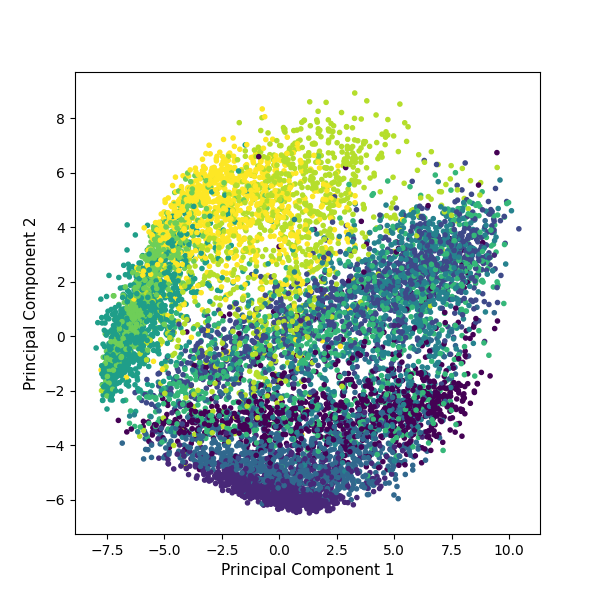
\includegraphics[width=0.4\textheight]{pca_linear_2comps.png}
		\label{fig:pca_linear_2comps}
	\end{subfigure}
	\begin{subfigure}{0.5\textwidth}
		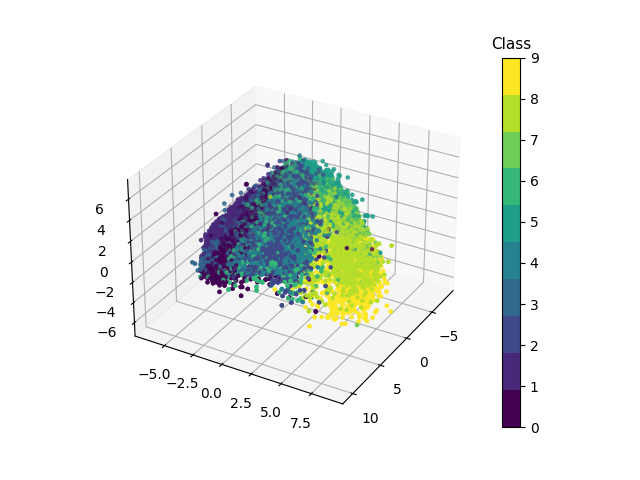
\includegraphics[width=0.4\textheight]{pca_linear_3comps.png}
		\label{fig:lpca_linear_3comps}
	\end{subfigure}
	\caption{First two and three principal components obtained by performing linear PCA, plotted along with true labels}
	\label{fig:pca_linear}
\end{figure}

Performing Kernel PCA with a Radial Basis Function kernel, using the default value of the dispersion parameter %is gamma the dispersion parameter?
 $\gamma = 1/\mathrm{\# samples} = 1/784$ , does not leed to better results, since the classes are still very mixed up, as we can see in Figure \ref{fig:pca_rbf}.
 
\begin{figure}[h]
	\begin{subfigure}{0.5\textwidth}
		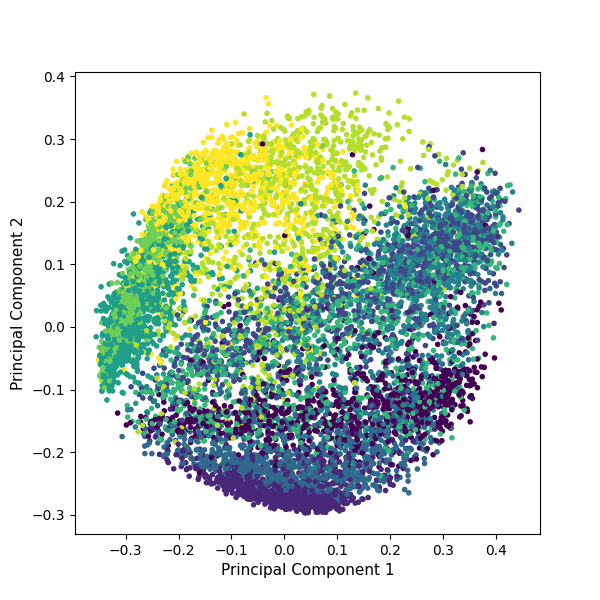
\includegraphics[width=0.4\textheight]{pca_rbf_2comps.png}
		\label{fig:pca_rbf_2comps}
	\end{subfigure}
	\begin{subfigure}{0.5\textwidth}
		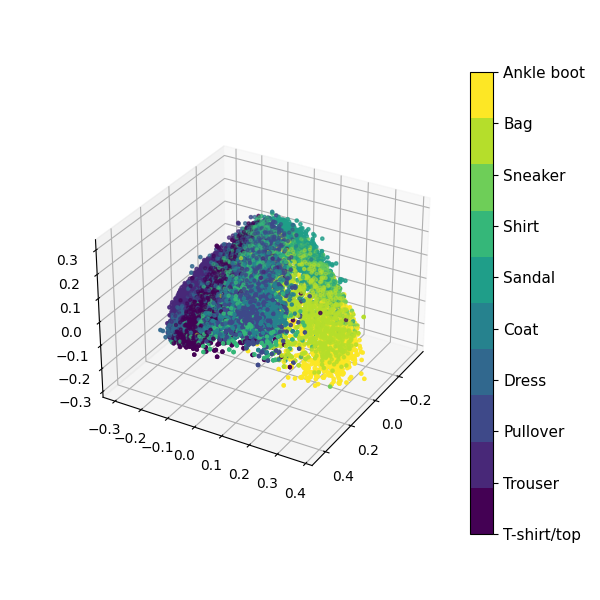
\includegraphics[width=0.4\textheight]{pca_rbf_3comps.png}
		\label{fig:pca_rbf_3comps}
	\end{subfigure}
	\caption{First two and three principal components obtained by performing kernel PCA with RBF kernel, plotted along with true labels}
	\label{fig:pca_rbf}
\end{figure}
%% Talk about parameter tuning
We tried two other kernels, but none of them separates clearly the clusters. In particular, looking at the three-components plots,  it seems that datapoints with labels 9, 8, 6 and 1 (Ankle boot, Bag, Shirt and T-Shirt/Top) are easyer to separate, while the others are mixed up.
\begin{figure}[h]
	\begin{subfigure}{0.5\textwidth}
		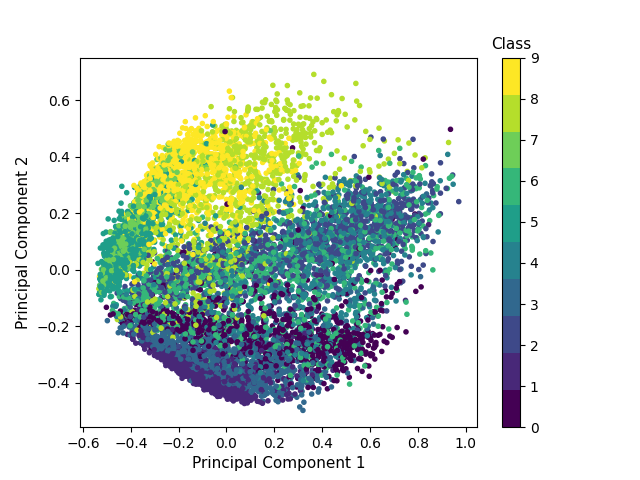
\includegraphics[width=0.4\textheight]{pca_poly_2comps.png}
		\caption{}
		\label{fig:pca_poly_2comps}
	\end{subfigure}
	\begin{subfigure}{0.5\textwidth}
		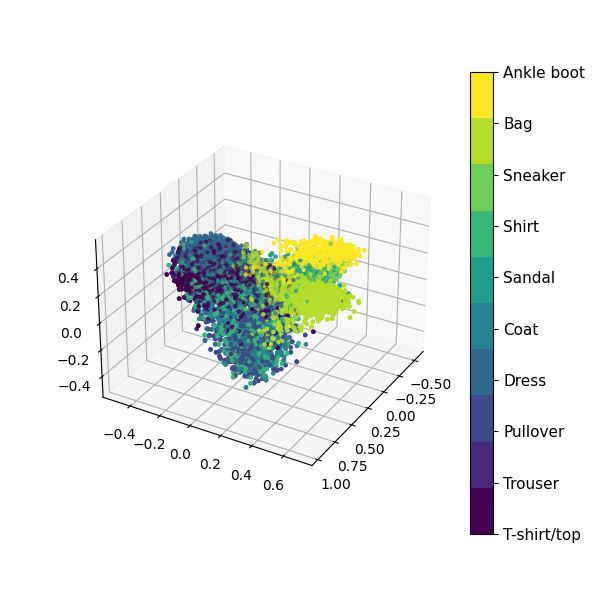
\includegraphics[width=0.4\textheight]{pca_poly_3comps.png}
		\caption{}
		\label{fig:pca_poly_3comps}
	\end{subfigure}
	\begin{subfigure}{0.5\textwidth}
		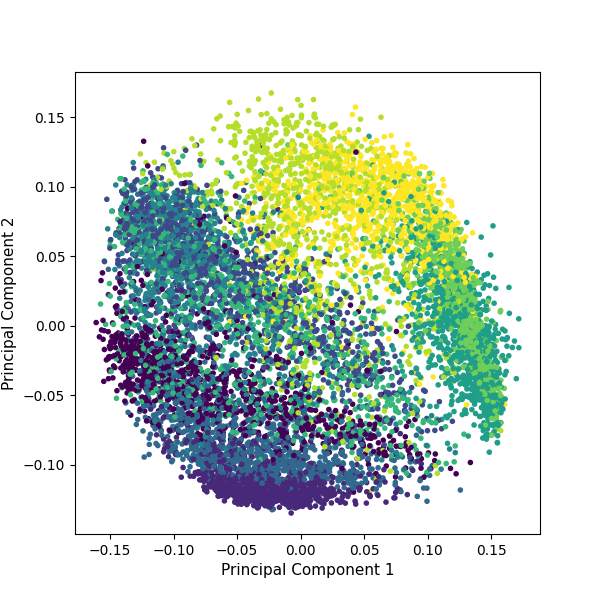
\includegraphics[width=0.4\textheight]{pca_sigmoid_2comps.png}
		\caption{}
		\label{fig:pca_sigmoid_2comps}
	\end{subfigure}
	\begin{subfigure}{0.5\textwidth}
		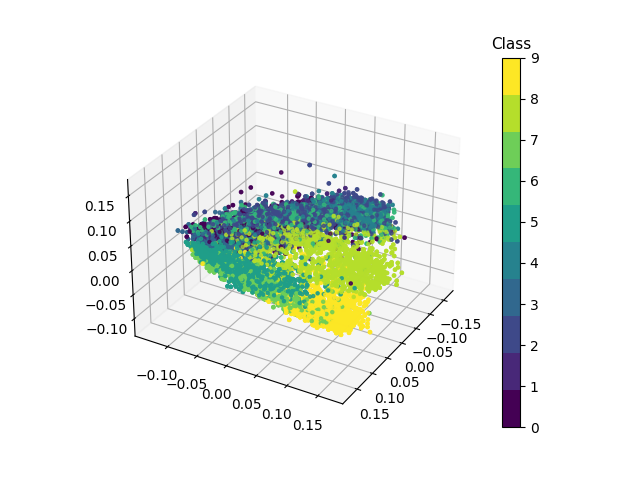
\includegraphics[width=0.4\textheight]{pca_sigmoid_3comps.png}
		\caption{}
		\label{fig:pca_sigmoid_3comps}
	\end{subfigure}
	\caption{First two and three principal components obtained by performing kernel PCA with polynomial (\ref{fig:pca_poly_2comps} and \ref{fig:pca_poly_3comps}) and sigmoid  (\ref{fig:pca_sigmoid_2comps} and \ref{fig:pca_sigmoid_3comps}) kernel, plotted along with true labels}
	\label{fig:pca_poly_sigmoid}
\end{figure}


\section{Exercise 2}
Even though no PCA method separates the datapoints in a satisfying way, we decided that the kernel PCA with sigmoid kernel is the one that works better. Then, we performed unsupervised clustering on those data, using three methods: K-means clustering, spectral clustering and Gaussian Mixture, obtaining the results showed in Figure

\begin{figure}[h]
	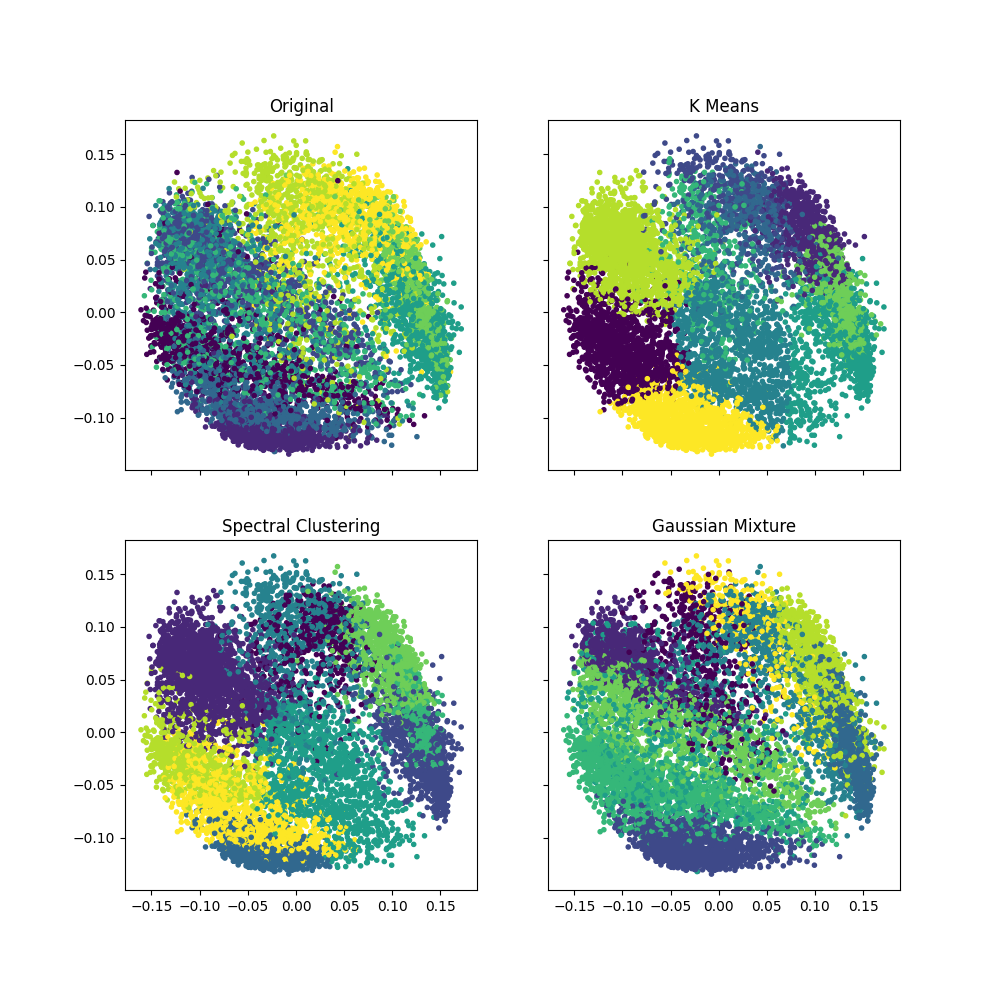
\includegraphics[width = 1 \textwidth]{unsupervised_clustering.png}
	\caption{}
	\label{fig:unsupervised_clustering}
\end{figure}



\section{Results}
% Your content goes here

\section{Conclusion}
% Your content goes here

% References if needed
% \bibliographystyle{plain}
% \bibliography{your_bibliography_file}

\end{document}
